% Completed CAL E1/E2 coupling analysis, transcribed from console.
% Plot source data are under report/maxcut/data; separate M5 held-out chapter follows.
\section{Coupling-matrix precision under nonideal p-bit response (completed CAL)}
\label{sec:cal-matrix}
\subsection{Research question and physical-numerical boundary}
This stage examines how low-order FP representations of the symmetric
coupling matrix $\mathbf J$ affect local-field accuracy, one-step
stochastic p-bit decision fidelity, and finite-budget weighted
Max-Cut quality under \emph{assumed} STT-MTJ-inspired nonidealities.
The original graph defines $J_{ij}=-w_{ij}$, $J_{ij}=J_{ji}$ and $J_{ii}=0$.
Each unique undirected coupling is encoded once and mirrored to obtain
$\widehat{\mathbf J}$, and the software computes
$\widehat{\mathbf H}=\widehat{\mathbf J}\mathbf s$
using adjacency lists and incremental updates. This is mathematically
matrix coupling, but it is not a fabricated $100\times100$ memory array.
Local-field accumulation is high-precision software arithmetic; the
p-bit voltage/pulse/DAC interface is represented by an illustrative
behavioural sigmoid, not by a bit-true physical implementation.

\begin{figure}[htbp]\centering
\begin{tikzpicture}[>=Latex, every node/.style={font=\small}, node distance=2.3mm]
\node[draw,rounded corners=2pt,fill=blue!6,minimum width=2.0cm,minimum height=1.15cm,align=center] (j) {Original $\mathbf J$\\$J_{ij}=-w_{ij}$};
\node[draw,rounded corners=2pt,fill=blue!6,minimum width=2.1cm,minimum height=1.15cm,align=center,right=of j] (q) {FP/INT encoded\\$\widehat{\mathbf J}$};
\node[draw,rounded corners=2pt,fill=blue!6,minimum width=2.1cm,minimum height=1.15cm,align=center,right=of q] (h) {Local field\\$\widehat{\mathbf H}=\widehat{\mathbf J}\mathbf s$};
\node[draw,rounded corners=2pt,fill=orange!9,minimum width=2.25cm,minimum height=1.15cm,align=center,right=of h] (p) {Nonideal p-bit\\$\sigma(2\beta H_i+\delta_i)$};
\node[draw,rounded corners=2pt,fill=gray!8,minimum width=2.0cm,minimum height=1.15cm,align=center,right=of p] (c) {Original-weight\\Max-Cut score};
\draw[->,thick] (j)--(q);\draw[->,thick](q)--(h);\draw[->,thick](h)--(p);\draw[->,thick](p)--(c);
\end{tikzpicture}
\caption{Coupling-matrix computation. Coupling \emph{coefficient} precision
is varied; accumulator and p-bit input-interface precision are separate,
currently idealised modeling assumptions.}\label{fig:coupling-pipeline}
\end{figure}

\subsection{Literature, format selection and model provenance}
Coupling errors can alter local extrema and update dynamics even when the
true optimum remains unchanged~\cite{PbitHizzani2026};
optimum-preserving QUBO compression requires more than small coefficient
MSE~\cite{PbitMuecke2025}. Floating-point Ising coefficients and
fixed-point coupling memories already exist~\cite{PbitTao2023,S33,S32}.
P-bit gain/offset mismatch and coupling-matrix-based compensation have
also been studied~\cite{PbitZhang2025}.
Measured pulse-driven STT-MTJ switching curves and calibration support
the physical motivation~\cite{PbitYang2502026}, but do not supply our
assumed 100-device post-calibration residual distribution.

FP4 E2M1 and FP6 E3M2 \emph{element sets} have a format precedent in
the OCP MX specification~\cite{PbitOCPMX2023}, but the existing
experiments use one coefficient-MSE-fitted \emph{global binary32 scale},
not the MX32 block-microscaling organisation. FP5 is custom; the
finite-only FP8 E4M3 implementation has unscaled maximum 480, versus
448 for OCP E4M3. The global-power-of-two-scale BFP control is limited
to that specific implementation. Coefficient MSE does not certify
original low-energy orderings or finite-budget search quality.

A sigmoid device model can be written
\begin{align}
P_i(+1\mid V)&=\sigma(a_i(V-V_{50,i})),\\
V&=V_{50,0}+2\beta(t)\widehat H_i/a_0,\\
P_i(+1)&=\sigma\left[(a_i/a_0)2\beta(t)\widehat H_i+
  a_i(V_{50,0}-V_{50,i})\right].
\end{align}
The gain ratio and logit offset can represent switching-slope and
midpoint mismatches, respectively; this is algebra, not device fitting.
The completed E2 offset-only experiments use gain exactly 1, one fixed
synthetic population $\delta_i=d v_i$ with $v_i\in[-1,1]$, and
scout-selected $d\in\{0.8,1.6\}$ logit on both CAL graphs.
These are diagnostic assumed stresses, not measured STT-MRAM
voltages, yield or post-calibration variability.

\subsection{Completed CAL solver-quality results}
The frozen solver uses 50,000 attempted linear-schedule Gibbs updates
and 24 paired seeds; it returns the earliest minimum
\emph{represented}-energy state and scores the \emph{original}
weighted Max-Cut. After the 240-new-run FP64 offset scout, exactly
576 new FP4/5/6 and INT4/5/6 offset runs completed.
The preregistered rule triggered 192 further FP8/INT8 runs.
Existing ideal E1 and 96 matched FP64 scout references were reused.
The 95\% paired-seed CI upper bounds must both meet the predeclared
conditions: absolute original-optimum gap at most 5\%, and extra
same-offset loss relative to FP64 at most $+1$ percentage point.
Failing to certify this conjunction does not prove a $>7.5\%$
absolute failure regime.

% CIs are deliberately incomplete: only original scout summary or documented terminal bounds.
\pgfplotsset{calquality/.style={
 width=.47\linewidth,height=5.35cm,ymin=2.4,ymax=9.0,xmin=-.5,xmax=8.5,
 xtick={0,1,2,3,4,5,6,7,8},
 xticklabels={FP64,FP4,FP5,FP6,FP8,INT4,INT5,INT6,INT8},
 x tick label style={rotate=47,anchor=east,font=\tiny},
 tick label style={font=\footnotesize},
 title style={font=\small},ylabel style={font=\small},
 grid=major,grid style={gray!18},mark size=1.65pt,
}}
\newcommand{\CALplot}[1]{%
\addplot+[only marks,mark=diamond*,color=gray!75,forget plot]
 table[col sep=comma,x=idx,y=#1mean]{report/maxcut/data/cal_quality_ref.csv};
\addplot+[only marks,mark=*,color=blue!75!black,forget plot]
 table[col sep=comma,x=idx,y=#1mean]{report/maxcut/data/cal_quality_fp.csv};
\addplot+[only marks,mark=square*,color=orange!85!black,forget plot]
 table[col sep=comma,x=idx,y=#1mean]{report/maxcut/data/cal_quality_int.csv};
\addplot+[only marks,mark=none,color=black!75,forget plot,
 error bars/.cd,y dir=both,y explicit]
 table[col sep=comma,x=idx,y=mean,
 y error plus expr=\thisrow{hi}-\thisrow{mean},
 y error minus expr=\thisrow{mean}-\thisrow{lo}]
 {report/maxcut/data/cal_ci_#1.csv};
\addplot+[red!70!black,dashed,domain=-.5:8.5,samples=2,forget plot]{5};
}
\begin{figure}[htbp]\centering
\begin{tikzpicture}
\begin{groupplot}[
 group style={group size=2 by 2,horizontal sep=1.5cm,vertical sep=2.15cm},
 calquality]
\nextgroupplot[title={Sparse, $d=0.8$},ylabel={Gap (\%)}]
\CALplot{s08}
\nextgroupplot[title={Sparse, $d=1.6$}]
\CALplot{s16}
\nextgroupplot[title={Dense, $d=0.8$},ylabel={Gap (\%)}]
\CALplot{d08}
\nextgroupplot[title={Dense, $d=1.6$}]
\CALplot{d16}
\end{groupplot}
\end{tikzpicture}
\caption{Original-weight Max-Cut gap means (24 matched seeds per
condition). Black diamonds: FP64; blue circles: FP; orange squares:
INT. Black whiskers show 95\% seed-bootstrap intervals \emph{only for
15 of 36 entries with accessible provenance}: FP64 intervals come from
the archived scout summary; selected lower-width intervals from
archived terminal reports (rounded). Points without whiskers lack
verified CI information \emph{in this report}; their uncertainty is not
zero. Different archived summary procedures may use different
bootstrap seeds. The dashed line is the 5\% absolute-gap target;
eligibility also requires the separate matched-FP64 $+1$
percentage-point quantisation screen. One synthetic device population,
not a physical yield claim.}
\label{fig:cal-offset-quality}
\end{figure}

On sparse $d=0.8$, FP4, INT5, INT6 and INT8 met the two
prespecified eligibility screens, but FP8 did not (paired
quantisation-penalty upper CI $+1.20$ pp). At sparse $d=1.6$
and both dense offset levels, no tested representation certified
both conditions; even the FP64 reference did not certify the 5\%
absolute target. On dense $d=1.6$, FP6/INT6 had mean original-cut
gaps 4.892\%/5.666\%; this does not establish a universal FP
advantage. All 12 offset-induced FP-minus-INT interaction confidence
intervals for widths 4/5/6 included zero; direct format differences
cannot be called proven offset interactions. Contrasts were
inspected without family-wise multiplicity correction.

\subsection{Coupling local-field and one-step probability diagnostics}
The read-only snapshot diagnostic evaluates nine representations on
the \emph{same 144 FP64-returned states} at static beta multipliers
0.5, 1 and 2. Its 3888 derived records are not 3888 independent
experimental trials, and \emph{no} new annealing runs were launched.
For matched state, offset and beta:
\begin{align}
\Delta H_i(\mathbf s)&=\sum_j(\widehat J_{ij}-J_{ij})s_j,\\
\Delta P_i&=\sigma(2\beta\widehat H_i+\delta_i)
             -\sigma(2\beta H_i+\delta_i).
\end{align}
For a \emph{single} update using the same uniform random draw,
$\Pr(\text{quantised decision}\ne\text{FP64 decision})=|\Delta P_i|$.
The sigmoid derivative is at most $1/4$, giving
$|\Delta P_i|\le\beta|\Delta H_i|/2$. This one-step result
cannot be multiplied by 50,000 to estimate wrong updates along
diverging full trajectories.

\begin{figure}[htbp]\centering
\begin{tikzpicture}
\begin{groupplot}[
 group style={group size=2 by 1,horizontal sep=1.4cm},
 width=.48\linewidth,height=5.6cm,
 xlabel={Relative RMS $\Delta H$ (\%)},ylabel={Mean $|\Delta P|$},
 tick label style={font=\footnotesize},label style={font=\footnotesize},
 title style={font=\small},grid=major,grid style={gray!18},
 ymin=0,ymax=.031,xmin=0,xmax=18]
\nextgroupplot[title={Sparse, $d=1.6$}]
\addplot+[only marks,mark=*,color=blue!75!black,mark size=2.5pt]
 table[col sep=comma,x=rel_rms_pct,y=abs_dP]{report/maxcut/data/cal_snap_sparse_fp.csv};
\addplot+[only marks,mark=square*,color=orange!85!black,mark size=2.5pt]
 table[col sep=comma,x=rel_rms_pct,y=abs_dP]{report/maxcut/data/cal_snap_sparse_int.csv};
\nextgroupplot[title={Dense, $d=1.6$},ylabel={}]
\addplot+[only marks,mark=*,color=blue!75!black,mark size=2.5pt]
 table[col sep=comma,x=rel_rms_pct,y=abs_dP]{report/maxcut/data/cal_snap_dense_fp.csv};
\addplot+[only marks,mark=square*,color=orange!85!black,mark size=2.5pt]
 table[col sep=comma,x=rel_rms_pct,y=abs_dP]{report/maxcut/data/cal_snap_dense_int.csv};
\node[font=\tiny,anchor=west] at (axis cs:3.991,.00384) {FP6};
\node[font=\tiny,anchor=west] at (axis cs:1.845,.00640) {INT8};
\end{groupplot}
\end{tikzpicture}
\caption{Static, state-conditioned local-field error and
switching-probability distortion on common FP64-returned states,
$d=1.6$ logit, beta multiplier 2. Blue circles: FP; orange squares:
INT. These are \emph{not observed annealing decision errors}.}
\label{fig:cal-error-propagation}
\end{figure}

For dense $d=1.6$, FP6 had relative RMS field error 3.991\%
and mean $|\Delta P|=0.00384$; INT6 had 5.347\% and 0.01369.
INT8 had \emph{smaller} RMS error than FP6 (1.845\%) but
\emph{larger} mean $|\Delta P|$ (0.00640), consistent with
sensitivity to where an error lies on the sigmoid.
FP8 reduced mean $|\Delta P|$ further to 0.00181, but its
separate solver gap was 5.363\% versus FP6's 4.892\%.
The one-step metrics are computed on common FP64 reference states
while final gaps come from \emph{different stochastic solver
trajectories}. This association is not causal proof that a
particular distortion caused a difference in final quality.

\begin{figure}[htbp]\centering
\begin{tikzpicture}
\begin{axis}[
 width=.86\linewidth,height=6.4cm,
 xlabel={Static mean $|\Delta P|$ at common FP64 states},
 ylabel={Separate solver original-optimum gap (\%)},
 xmin=-.001,xmax=.031,ymin=4.35,ymax=8.25,
 grid=major,grid style={gray!18},
 tick label style={font=\footnotesize},label style={font=\small},
 legend style={at={(.97,.97)},anchor=north east,font=\footnotesize}]
\addplot+[only marks,mark=*,mark size=2.3pt,color=blue!75!black]
 table[col sep=comma,x=abs_dP,y=solver_gap]
 {report/maxcut/data/cal_snap_dense_fp.csv};
\addlegendentry{FP}
\addplot+[only marks,mark=square*,mark size=2.3pt,color=orange!85!black]
 table[col sep=comma,x=abs_dP,y=solver_gap]
 {report/maxcut/data/cal_snap_dense_int.csv};
\addlegendentry{INT}
\addplot+[red!70!black,dashed,domain=-.001:.031,samples=2,forget plot]{5};
\node[font=\scriptsize,anchor=west] at (axis cs:.00384,4.892) {FP6};
\node[font=\scriptsize,anchor=west] at (axis cs:.01369,5.666) {INT6};
\node[font=\scriptsize,anchor=west] at (axis cs:.00181,5.363) {FP8};
\end{axis}
\end{tikzpicture}
\caption{Dense CAL at $d=1.6$ logit: static mean probability mismatch
versus the \emph{separately run} finite-budget solver's original-cut
gaps. The x-axis uses common FP64-returned states, whereas the y-axis
comes from representation-specific trajectories. This association
does not establish a causal mechanism.}
\label{fig:static-vs-quality}
\end{figure}

\begin{figure}[htbp]\centering
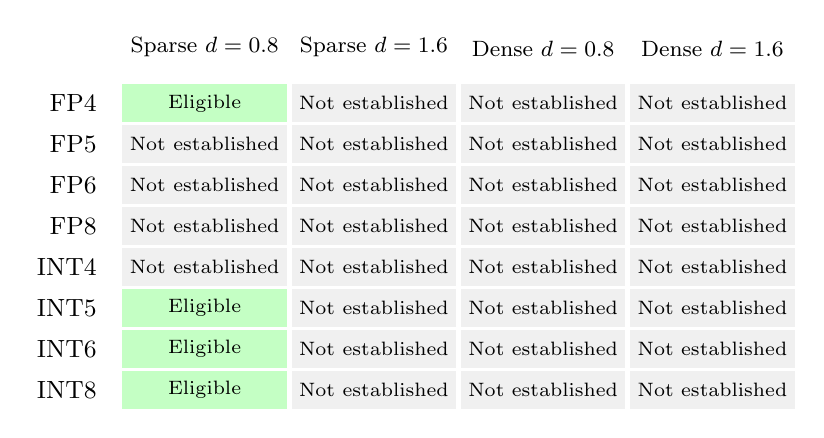
\begin{tikzpicture}[x=2.15cm,y=.52cm]
\foreach \c/\heading in {0/{Sparse $d=0.8$},1/{Sparse $d=1.6$},2/{Dense $d=0.8$},3/{Dense $d=1.6$}}{
  \node[font=\footnotesize,anchor=south] at (\c+1,0.35) {\heading};
}
\foreach \r/\fmt in {0/FP4,1/FP5,2/FP6,3/FP8,4/INT4,5/INT5,6/INT6,7/INT8}{
  \node[font=\small,anchor=east] at (.42,-\r-.55) {\fmt};
  \foreach \c in {0,1,2,3}{
    \node[draw=white,fill=gray!12,minimum width=2.1cm,
       minimum height=.49cm,font=\scriptsize,inner sep=1pt]
       at (\c+1,-\r-.55) {Not established};
  }
}
\foreach \r in {0,5,6,7}{
  \node[draw=white,fill=green!23,minimum width=2.1cm,
    minimum height=.49cm,font=\scriptsize,inner sep=1pt]
       at (1,-\r-.55) {Eligible};
}
\end{tikzpicture}
\caption{Frozen conditional precision eligibility across four CAL
offset conditions. A format is eligible only when both 95\% upper
confidence bounds certify the 5\% absolute-gap screen and the
$+1$ percentage-point quantisation-penalty screen. An unestablished
result is \emph{not} proof of an absolute failure regime. These criteria
describe only two named graphs and one synthetic device population.}
\label{fig:cal-precision-eligibility}
\end{figure}

\subsection{FYP inference and held-out hypothesis}
The CAL evidence supports bounded format--response tradeoffs, not
a universal FP/INT bit-width rule, measured silicon variability,
or full-chip implementation savings. The two 100-spin
\texttt{\_7777} held-out graphs remain untouched.
Before testing them, the proposed dense-graph hypothesis is:
at beta multiplier 2, FP6 will have a lower paired-seed mean
same-offset absolute probability distortion than INT6 at each
of $d=0.8$ and $1.6$. The held-out quality comparison must be
reported separately; lower static $|\Delta P|$ does not guarantee
better finite-budget Max-Cut quality. All original quality
thresholds, formats and source-only scale rules remain fixed.
